\documentclass[aspectratio=169]{beamer}
\setbeamertemplate{navigation symbols}{}
\usepackage{color,amsmath,comment, subfigure}
\usepackage{booktabs}
\usepackage{url}


%%%%%%%%%%%%%%%%%%%%%%%%%%
\title[]{Class 15: Complex contagion}
\author[]{Matthew J. Salganik}
\institute[]{Sociology 204: Social Networks\\Princeton University}
\date[]{
1/2 Simple and complex contagion
\vfill

\begin{flushleft}
\vspace{0.6in}

\includegraphics[width=0.1\textwidth]{figures/cc.png}
\end{flushleft}
}

\begin{document}
%%%%%%%%%%%%%%%%%%%%%%%%%%%
\frame{\titlepage}
%%%%%%%%%%%%%%%%%%%%%%%%%%%
\begin{frame}

\begin{center}
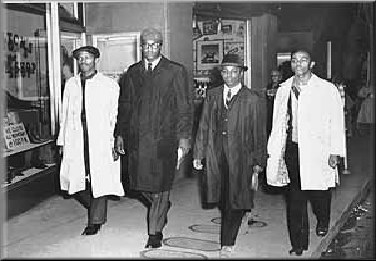
\includegraphics[width=0.5\textwidth]{figures/Greensboro_Four_Feb_1960}
\end{center}

Greensboro Four (L-R: David McNeil, Franklin McCain, Ezell Blair, Joseph McNeil)

\vfill
\tiny{\url{https://en.wikipedia.org/wiki/Greensboro_sit-ins\#/media/File:Greensboro_Four,_Feb_1960.jpg}}

\end{frame}
%%%%%%%%%%%%%%%%%%%%%%%%
\begin{frame}

Distinguish between:
\begin{itemize}
\item spread of information and disease
\item spread of behavior, especially high-risk activism
\end{itemize}

\end{frame}
%%%%%%%%%%%%%%%%%%%%%%%%
\begin{frame}

Two interrelated themes:
\begin{itemize}
\item How do things spread?
\item What does this network look like?
\end{itemize}

\vfill
Centola work builds on a lot of the things we read before spring break. I hope you could see that.

\end{frame}
%%%%%%%%%%%%%%%%%%%%%%%%%
\begin{frame}

\begin{center}
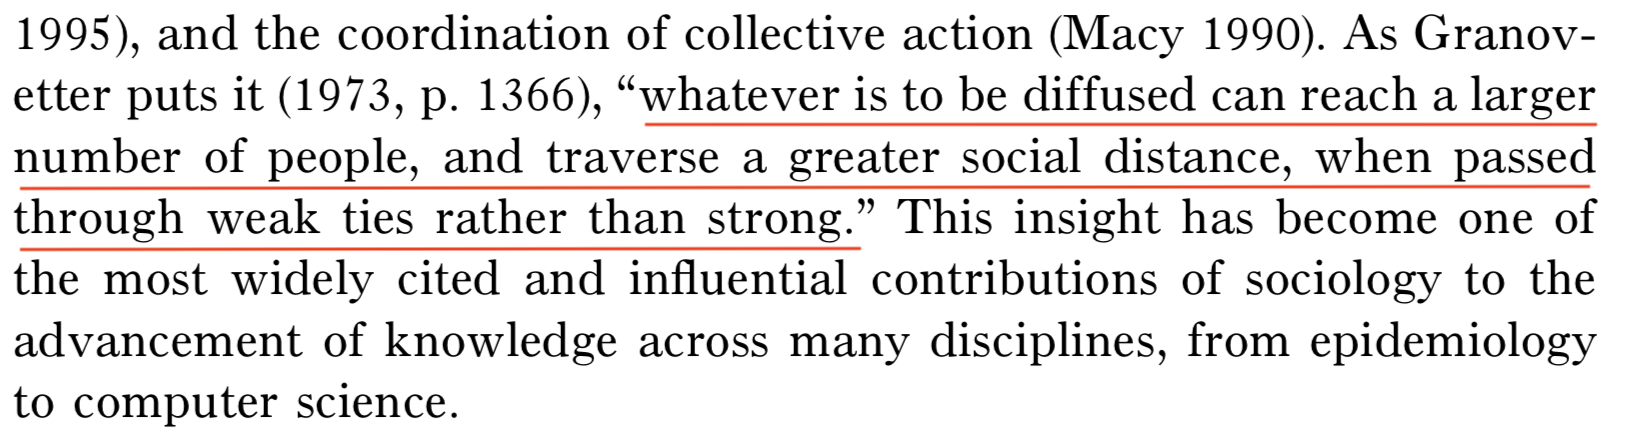
\includegraphics[width=\textwidth]{figures/centola_complex_2007_granovetter}
\end{center}

\vfill
What are the scope conditions for this claim?

\end{frame}
%%%%%%%%%%%%%%%%%%%%%%%%%%
\begin{frame}

\begin{itemize}
\item simple contagion: 1 source of contact may enable activation \onslide<3->{(disease)}
\pause
\item complex contagion: 2 or more sources of contact needed for activation \onslide<4>{(behavior)}
\end{itemize}

\end{frame}
%%%%%%%%%%%%%%%%%%%%%%%%%%
\begin{frame}

Threshold model 
$\tau = \frac{a}{z}$
where
\begin{itemize}
\item $\tau$ is the threshold
\item $a$ is the number of activated neighbors
\item $z$ is the degree
\end{itemize}

\vfill
$\tau = \frac{1}{8}$ is different from $\tau = \frac{6}{48}$
\end{frame}
%%%%%%%%%%%%%%%%%%%%%%%%%%
\begin{frame}

\begin{center}
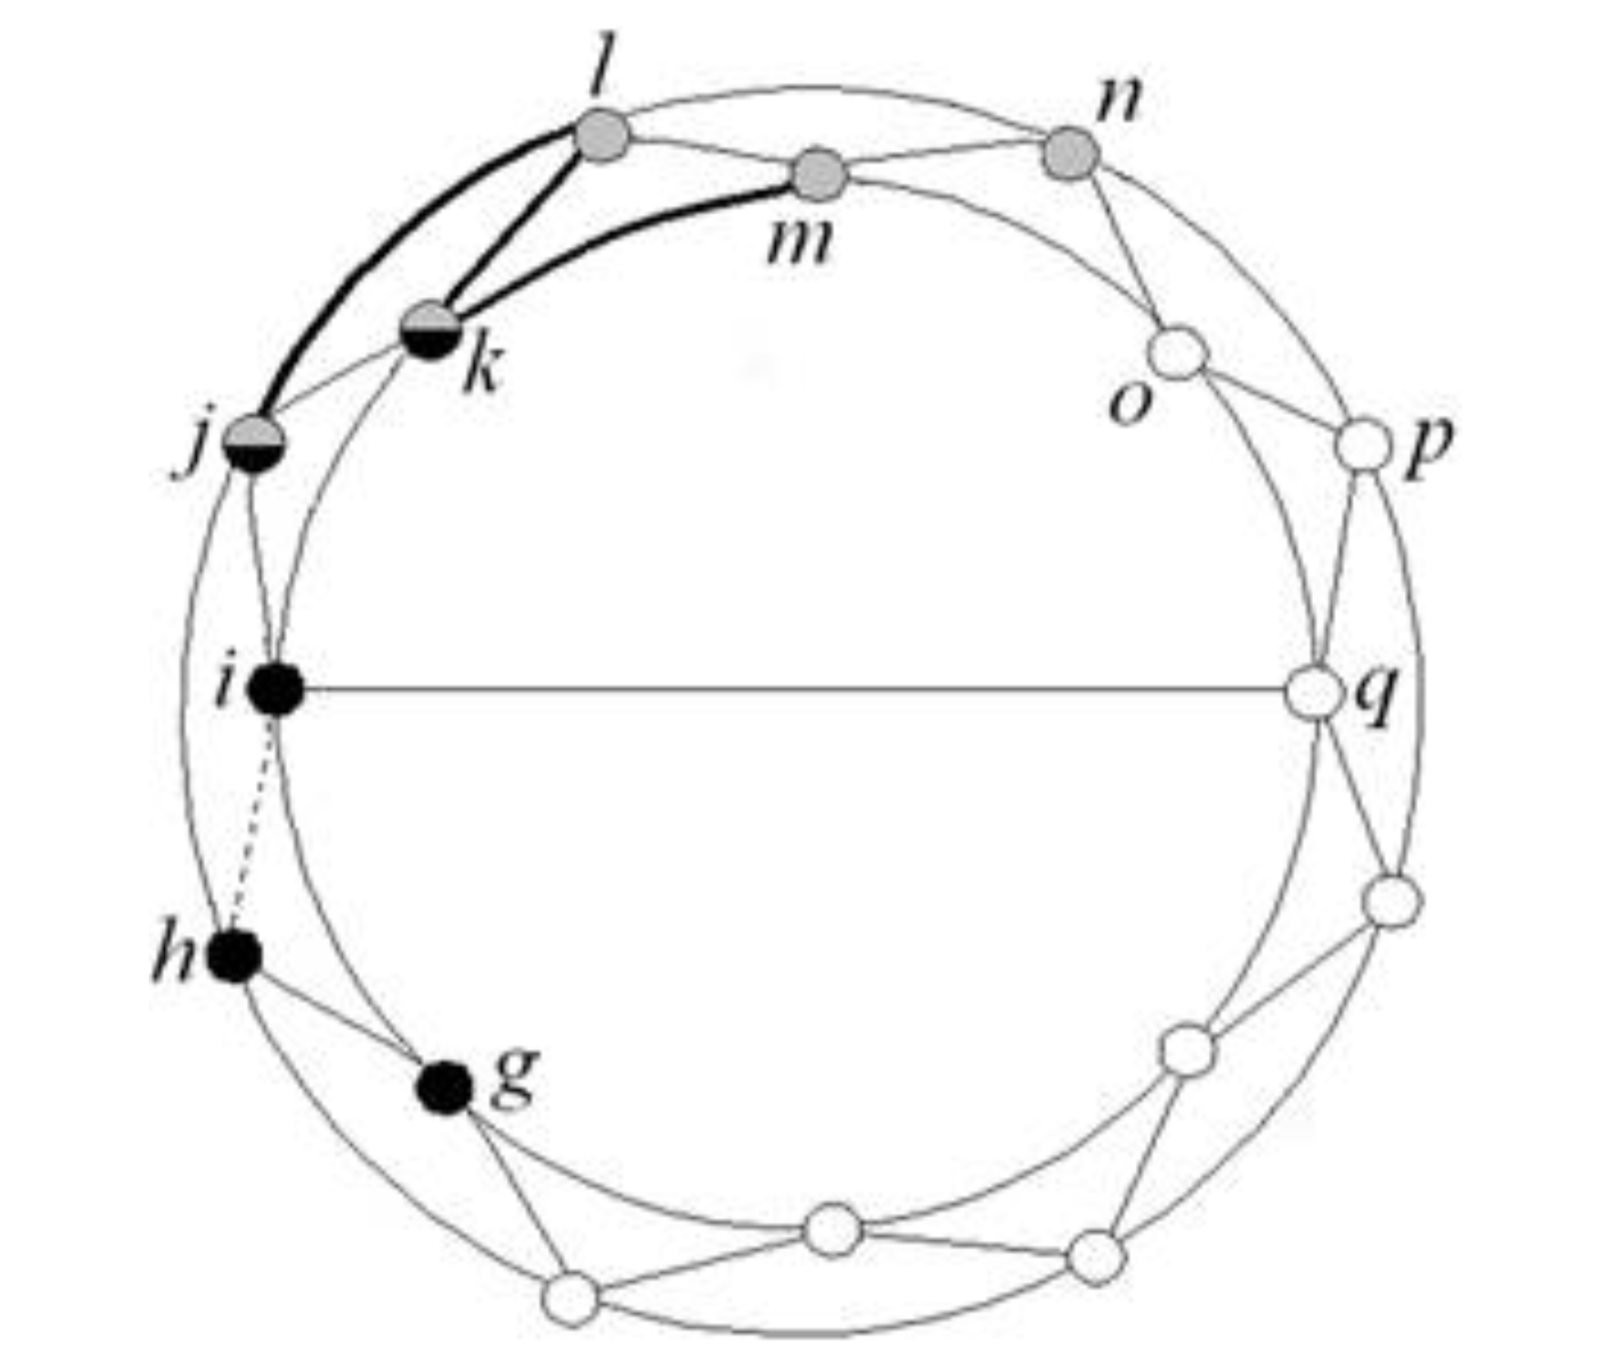
\includegraphics[width=0.4\textwidth]{figures/centola_complex_2007_fig1}
\end{center}

\begin{itemize}
\item Simple contagion: $l$ and $m$ are sick, \pause which infects $k$ \pause which infects $j$ \pause which infects $i$ \pause which infects $q$ and $h$ $\ldots$ \pause
\item Complex contagion ($\tau = 2/4$): $l$ and $m$ are protesting, \pause which activates $k$ \pause which activates $j$ \pause which activates $i$ \pause but does not activate $h$. \pause
\item Shortcuts that help with simple contagion cab block complex contagion
\end{itemize}

\end{frame}
%%%%%%%%%%%%%%%%%%%%%%%%
\begin{frame}

Granovetter talks about bridge \emph{length}

\begin{figure}
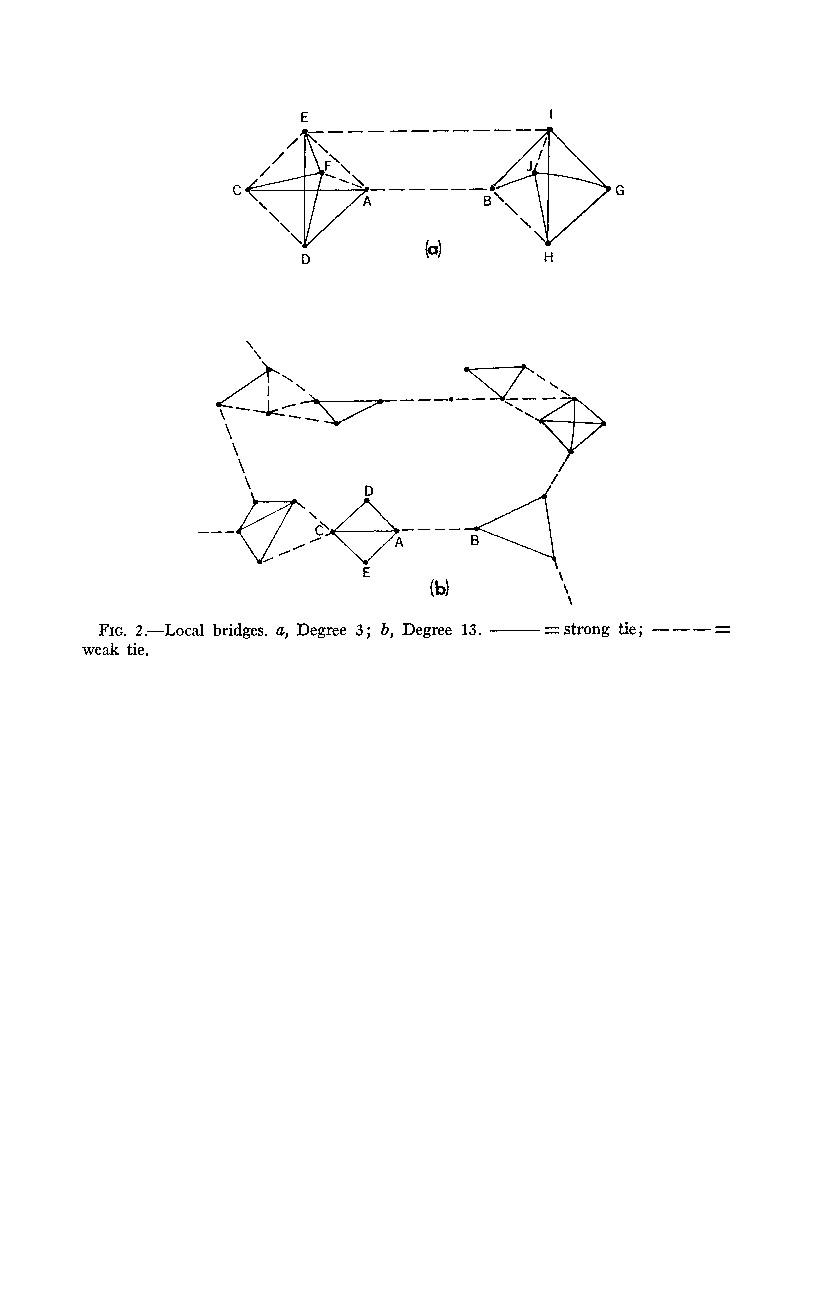
\includegraphics[width=0.6\textwidth]{figures/granovetter_strength_1973_fig2}
\end{figure}


\end{frame}
%%%%%%%%%%%%%%%%%%%%%%%%
\begin{frame}

Centola talks about bridge \emph{width}\\

\begin{figure}
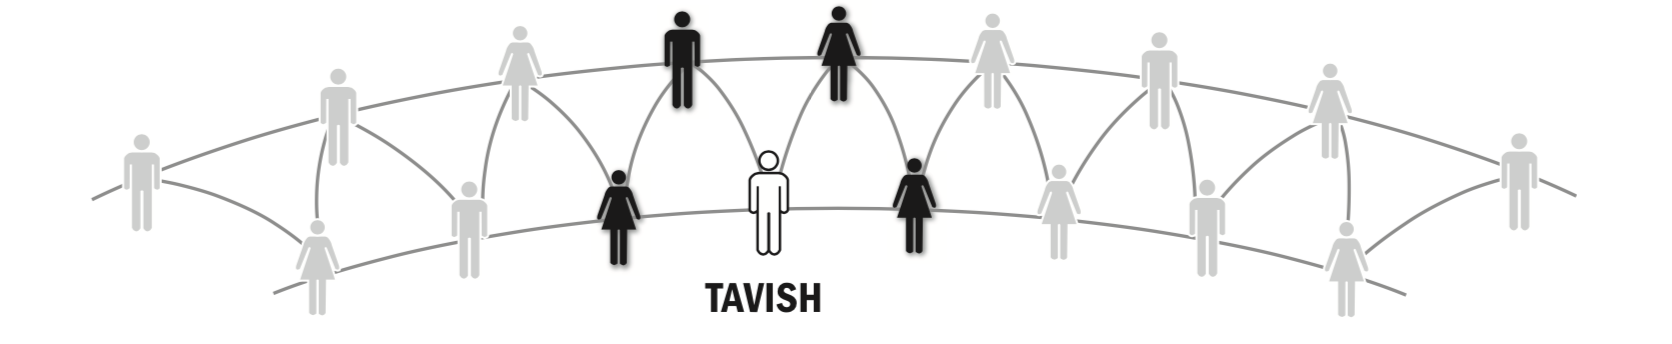
\includegraphics[width=0.5\textwidth]{figures/centola_how_2018_fig3_6}
\end{figure}

\pause

\begin{figure}
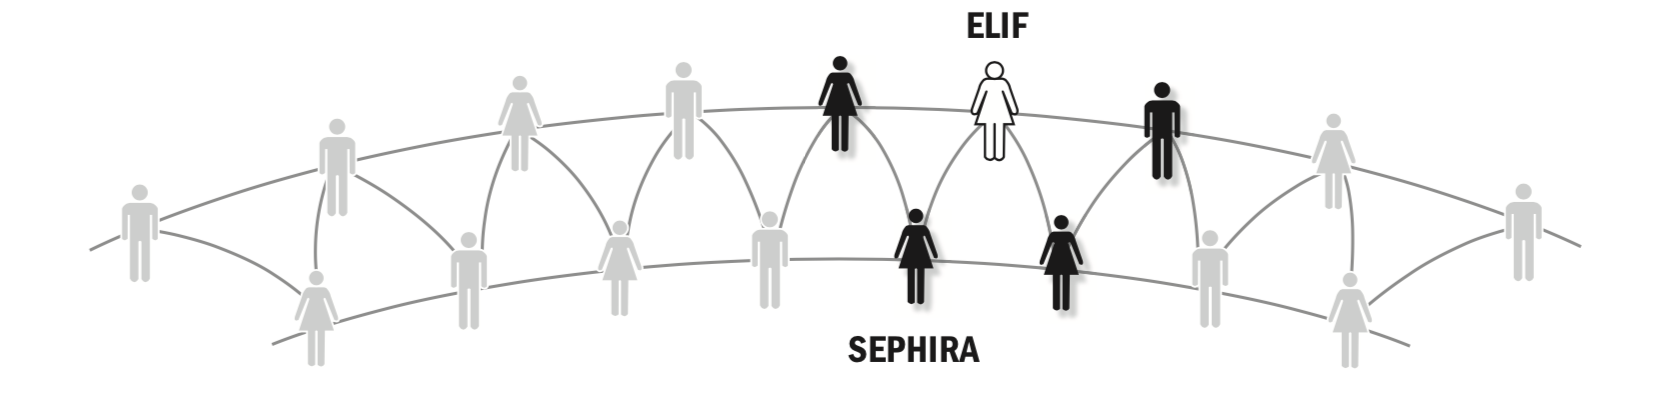
\includegraphics[width=0.5\textwidth]{figures/centola_how_2018_fig3_7}
\end{figure}

\pause

\begin{figure}
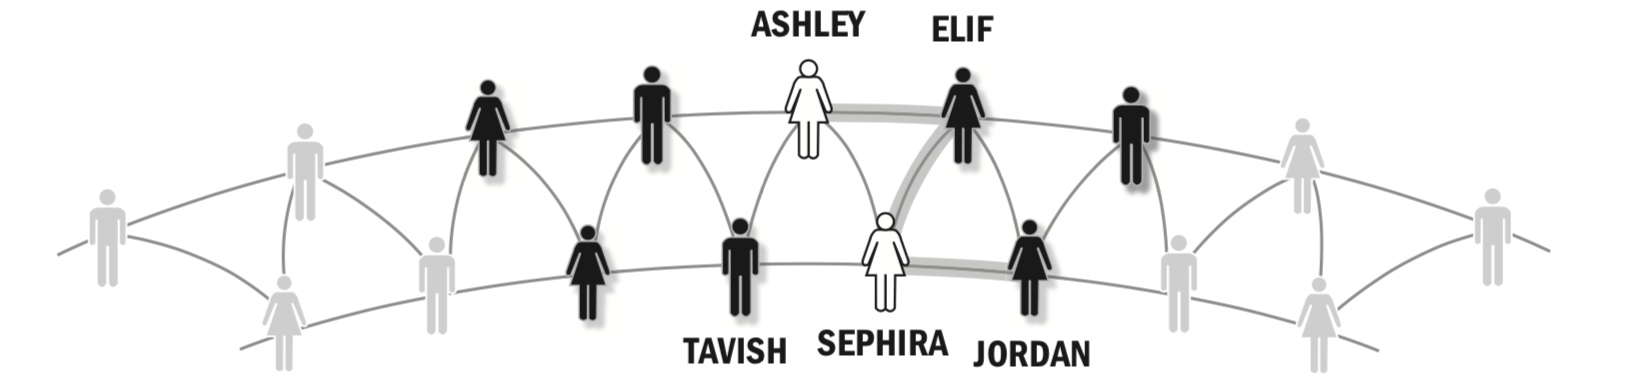
\includegraphics[width=0.5\textwidth]{figures/centola_how_2018_fig3_8}
\end{figure}

\pause

Ties between Tavish's neighborhood and Elif's neighborhood: 3 (bridge width)

\vfill
\tiny{Centola (2018)}
\end{frame}
%%%%%%%%%%%%%%%%%%%%%%%%
\begin{frame}

Creating shortcuts can hurt complex contagion if it breaks local redundancy \pause

\begin{figure}
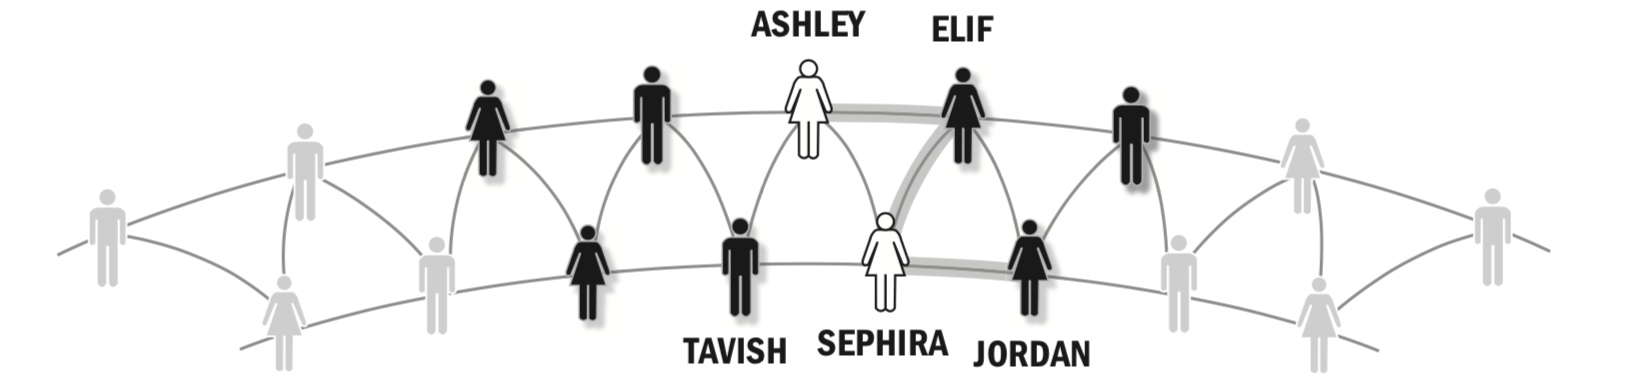
\includegraphics[width=0.5\textwidth]{figures/centola_how_2018_fig3_8}
\end{figure}

\begin{figure}
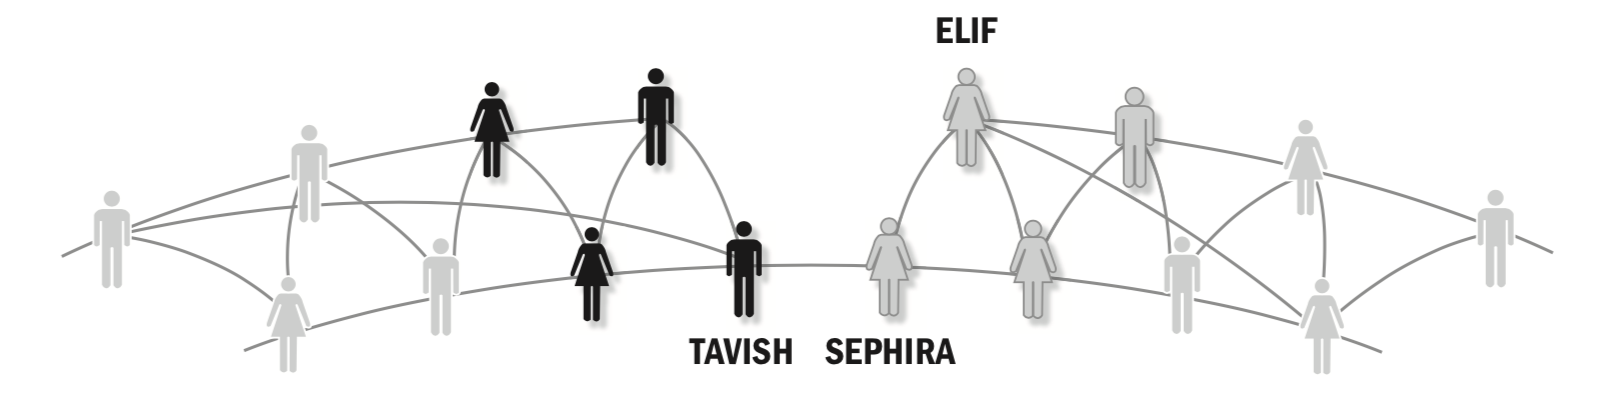
\includegraphics[width=0.5\textwidth]{figures/centola_how_2018_fig3_9}
\end{figure}

Ties between Tavish's neighborhood and Elif's neighborhood: 1 (bridge width)

\vfill
\tiny{Centola (2018)}
\end{frame}
%%%%%%%%%%%%%%%%%%%%%%%%
\begin{frame}

Next step: 
\begin{itemize}
\item Move from Ring lattice to two-dimensional lattice with Moore neighborhoods
\item Requires switch from analytic results to simulation.
\end{itemize}

\vfill
Here's an example of a two-dimensional lattice with Moore neighborhoods
\begin{figure}
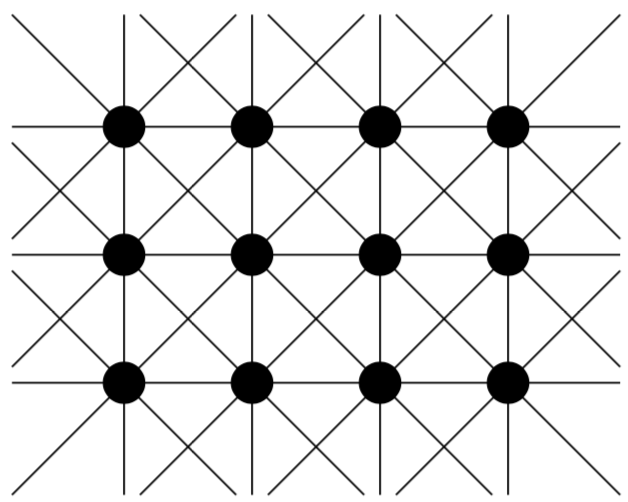
\includegraphics[width=0.3\textwidth]{figures/neary_heterogenity_2017_fig4b}
\end{figure}

\end{frame}
%%%%%%%%%%%%%%%%%%%%%%%%%%
\begin{frame}

\begin{figure}
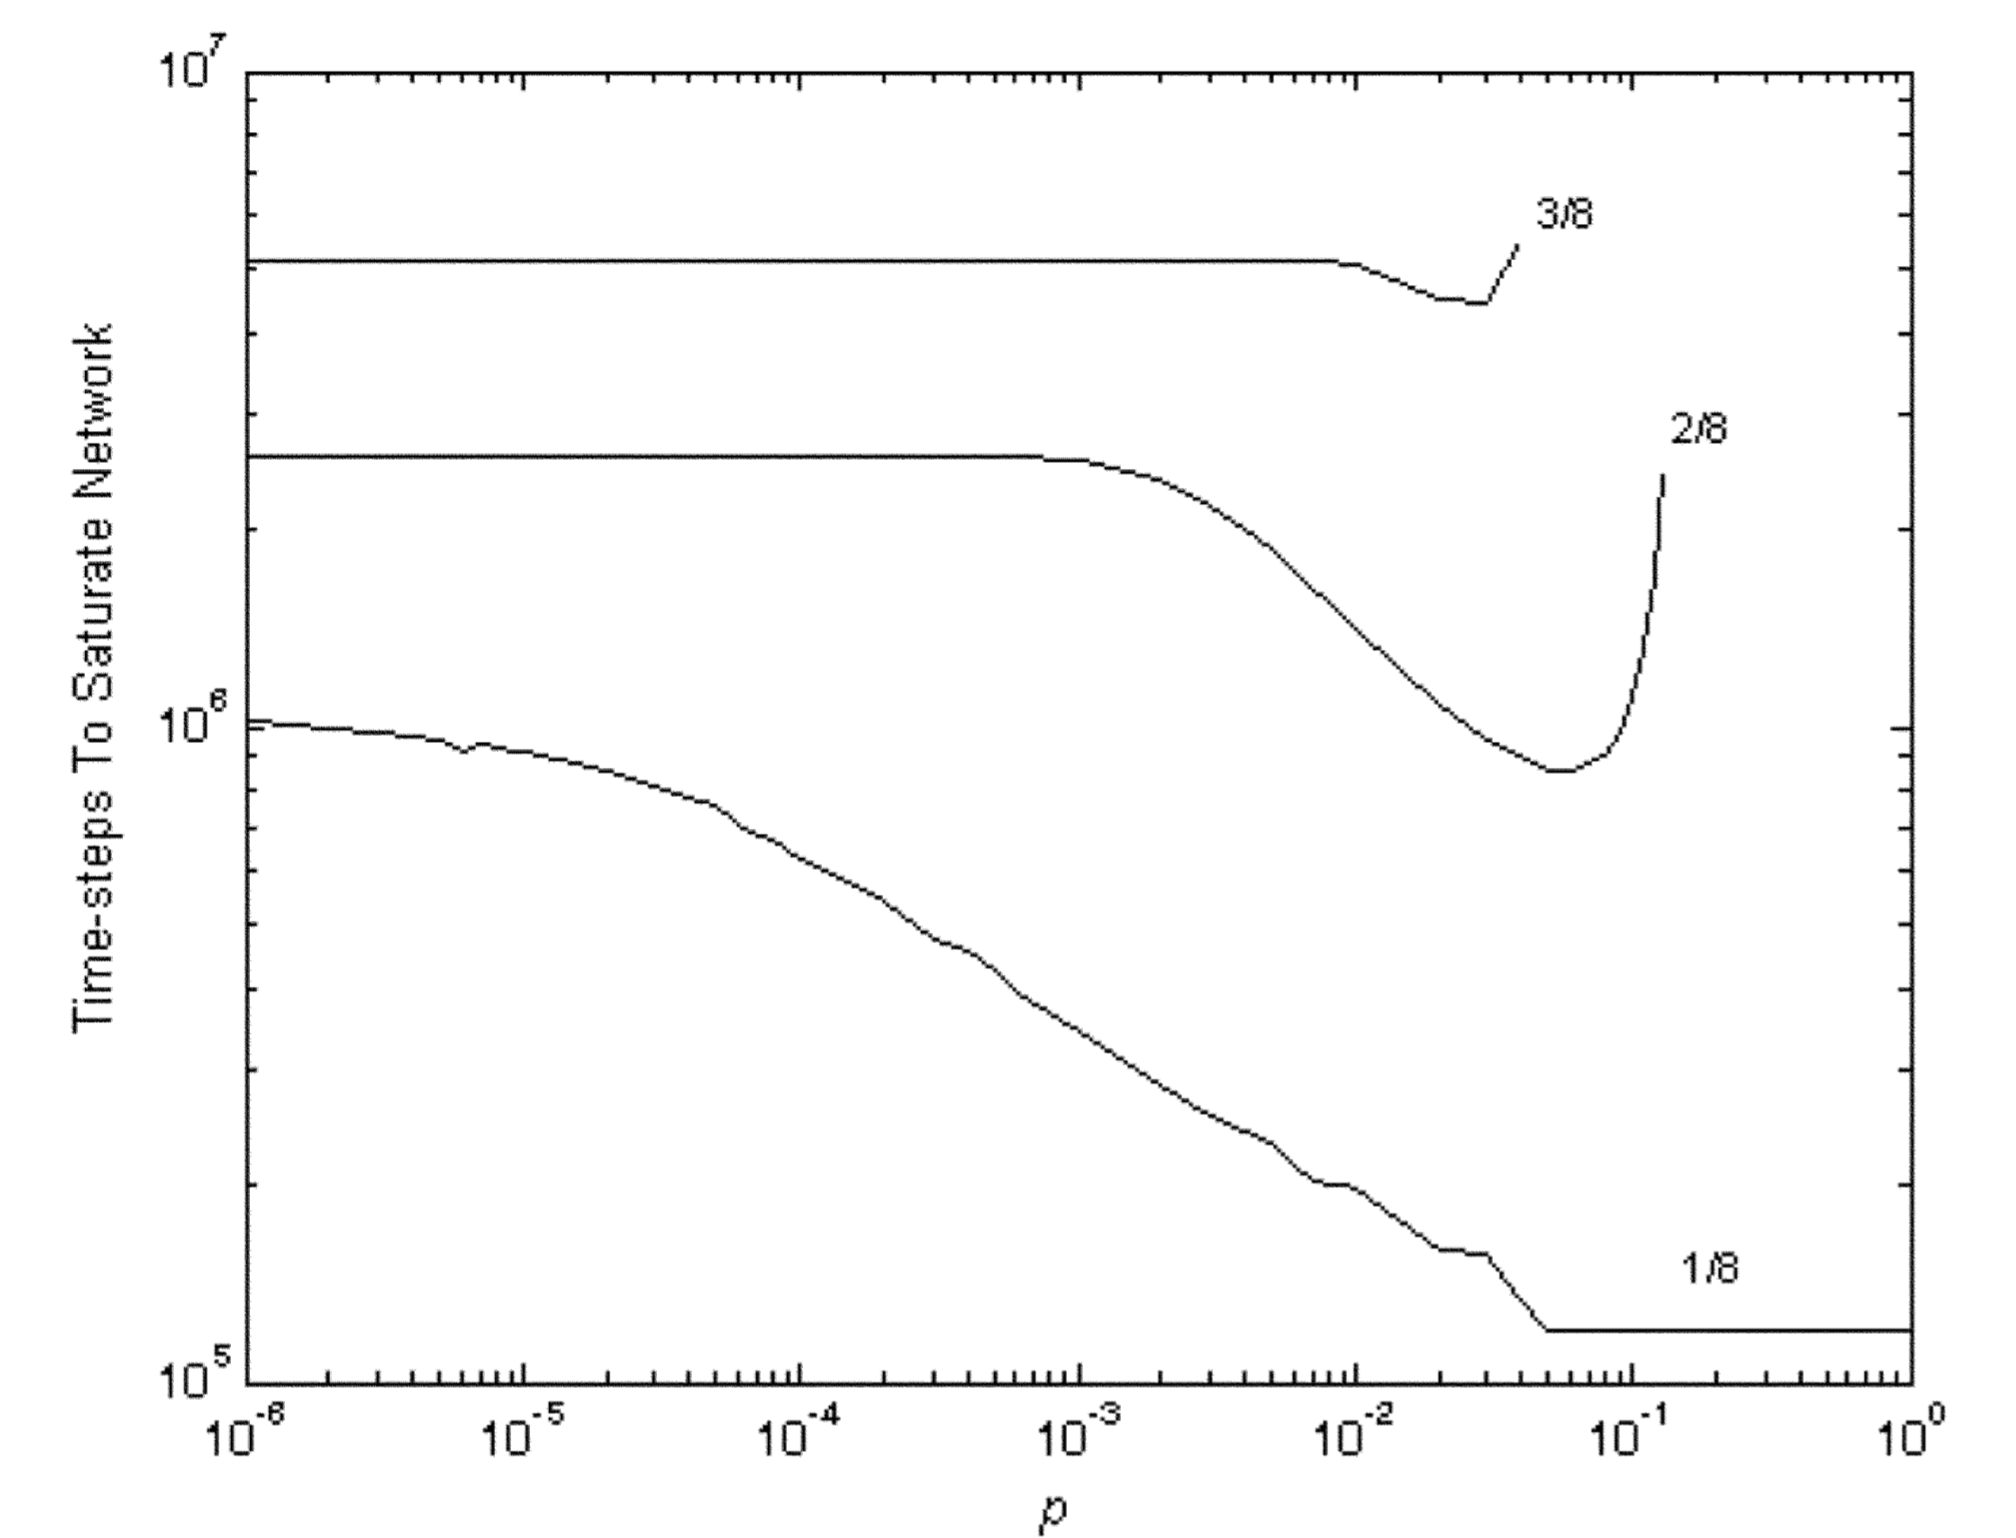
\includegraphics[width=0.45\textwidth]{figures/centola_complex_2007_fig3}
\end{figure}

\pause
\begin{itemize}
\item simple contagion acts as we expect based on Watts and Strogatz (1998) \pause
\item complex contagion does not benefit from low levels of rewiring \pause
\item increasing rewiring has a non-monotoic (U-shaped) impact on complex contagions \pause
\item as rewiring exceeds a critical upper limit, complex contagion fails entirely \pause
\end{itemize}
\vfill
Notice a research strategy of ``replicate and extend''

\end{frame}
%%%%%%%%%%%%%%%%%%%%%%%%%
\begin{frame}

Robustness results
\begin{itemize}
\item threshold heterogeneity
\item heterogeneity of influence
\item strong and weak ties
\item heterogeneity of degree
\end{itemize} 

\end{frame}
%%%%%%%%%%%%%%%%%%%%%%%%
\begin{frame}

Results in Centola and Macy are based on simple models, could something like this really happen?

\end{frame}

\end{document}
